% 图 6.29 二维磁体中的涡旋激发：圆盘内 M(r)=|M|(y cos(pi r/R) - x sin(pi r/R))，盘外 -y
\documentclass[tikz,border=5pt]{standalone}
\usetikzlibrary{arrows.meta}
\usepackage{amsmath}
\usepackage{bm}
\usepackage{fontspec}
\setmainfont{Times New Roman}
\begin{document}
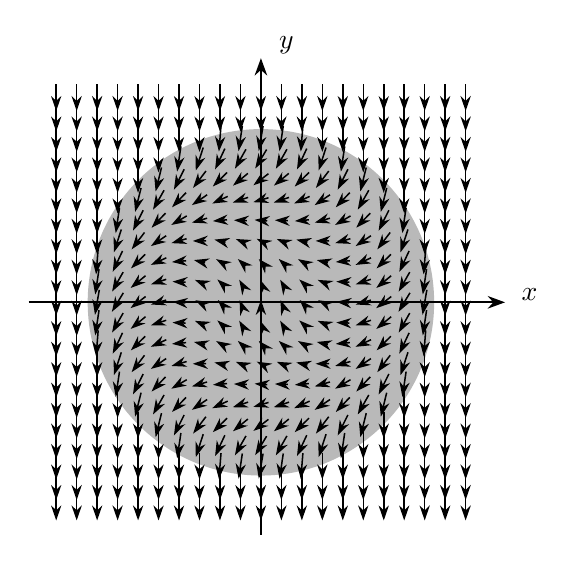
\begin{tikzpicture}[line width=0.8pt,>=Stealth,
  varr/.style={->,line width=0.55pt,>={Stealth[length=1.9mm,width=1.3mm]}}]
% grey disk
\fill[gray!55] (0,0) circle (2.2);
% axes
\draw[->,line width=0.7pt,>={Stealth[length=2.2mm,width=1.6mm]}] (-2.95,0) -- (3.1,0);
\node[anchor=west] at (3.18,0.1) {$x$};
\draw[->,line width=0.7pt,>={Stealth[length=2.2mm,width=1.6mm]}] (0,-2.95) -- (0,3.1);
\node[anchor=south west] at (0.1,3.02) {$y$};
% spin arrows on a grid
\foreach \i in {0,...,20} {
  \foreach \j in {0,...,20} {
    \pgfmathsetmacro{\xx}{-2.6+\i*0.26}
    \pgfmathsetmacro{\yy}{-2.6+\j*0.26}
    \pgfmathsetmacro{\rr}{sqrt(\xx*\xx+\yy*\yy)}
    \pgfmathsetmacro{\rn}{\rr/2.2}
    \ifdim\rn pt<0.985pt
      \pgfmathsetmacro{\angA}{90+180*\rn}
      \pgfmathsetmacro{\cA}{cos(\angA)}
      \pgfmathsetmacro{\sA}{sin(\angA)}
      \pgfmathsetmacro{\leng}{0.17*max(\rn,0.18)}
      \draw[varr] (\xx-\leng*\cA,\yy-\leng*\sA) -- (\xx+\leng*\cA,\yy+\leng*\sA);
    \else
      \draw[varr] (\xx,\yy+0.17) -- (\xx,\yy-0.17);
    \fi
  }
}
\end{tikzpicture}
\end{document}
